\documentclass[aspectratio=169,14pt,spanish]{beamer}

\usepackage[utf8]{inputenc}
\usepackage[T1]{fontenc}
\usepackage[spanish]{babel} % Changes theorem->teorema, proof->demostración...

%%%%%%%%%%%%%%%%%%%%%%%%%%%%%%%%%%%%%%%%%%%%%%%
%%%%%%%%%%%%%%%% CONFIGURATION %%%%%%%%%%%%%%%%
%%%%%%%%%%%%%%%%%%%%%%%%%%%%%%%%%%%%%%%%%%%%%%%

\usetheme{default}
\setbeamertemplate{navigation symbols}{} % Removes the navigation symbols :_)

% Opens the PDF document in full screen by default :)
%\hypersetup{pdfpagemode=FullScreen}

%Language
\selectlanguage{spanish}

%%%%%%%%%%%%%%%%%%%%%%%%%%%%%%%%%%%%%%%%%%%%%%%
%%%%%%%%%%%%%%%%%%%% TITLE %%%%%%%%%%%%%%%%%%%%
%%%%%%%%%%%%%%%%%%%%%%%%%%%%%%%%%%%%%%%%%%%%%%%

\title[Rectificación]{Rectificación de un par estéreo}
\subtitle[Implementación de Loop Zhang]{Implementación del algoritmo de Loop \& Zhang}
\author[A. A. Caballero, A. G. Montoro]{Antonio Álvarez Caballero, Alejandro García Montoro}
\institute[UGR]{Universidad de Granada}
\date{\today}

% Frame whenever a new section begins
\AtBeginSection[]{
    \begin{frame}[plain]
        \begin{center}
                \huge{\insertsection}
        \end{center}
    \end{frame}
}

% Frame whenever a new subsection begins
\AtBeginSubsection[]{
    \begin{frame}[plain]
        \begin{center}
                \huge{\insertsubsection}
        \end{center}
    \end{frame}
}


%%%%%%%%%%%%%%%%%%%%%%%%%%%%%%%%%%%%%%%%%%%%%%%
%%%%%%%%%%%%%%%%%%% COLORS %%%%%%%%%%%%%%%%%%%%
%%%%%%%%%%%%%%%%%%%%%%%%%%%%%%%%%%%%%%%%%%%%%%%

%%%%%%%%%%%%%%%% DECLARATIONS %%%%%%%%%%%%%%%%%

\definecolor{c_gray_l}{HTML}{FAFAFA} % background light gray
\definecolor{c_metal}{HTML}{37474F}  % background dark metal blue

%%%%%%%%%%%%%%%% DEFINITIONS %%%%%%%%%%%%%%%%%*

\setbeamercolor*{default}{
    bg=c_metal,
    fg=c_gray_l
}

\setbeamercolor*{palette primary}{
    parent=default
}

\setbeamercolor*{palette secondary}{
    bg=c_gray_l,
    fg=c_metal
}

\setbeamercolor*{background canvas}{
    parent = palette primary
}

\setbeamercolor*{normal text}{
    fg = c_gray_l
}

\setbeamercolor*{titlelike}{
    parent = palette secondary
}

\setbeamercolor*{section in toc}{
    parent = palette primary
}

\setbeamercolor*{block title alerted}{
    bg = red!60,
    fg = c_gray_l
}

\setbeamercolor*{block body alerted}{
    parent = palette secondary
}

%%%%%%%%%%%%%%%%%%%%%%%%%%%%%%%%%%%%%%%%%%%%%%%
%%%%%%%%%%%%%%%%%% DOCUMENT %%%%%%%%%%%%%%%%%%%
%%%%%%%%%%%%%%%%%%%%%%%%%%%%%%%%%%%%%%%%%%%%%%%

\begin{document}

    \titlepage

    \begin{frame}[t]{Contenidos}
        \tableofcontents
    \end{frame}
    %--- Next Frame ---%

    \section{Descripción del problema}

    \begin{frame}{Descripción del problema}{}
        %\alert{Una alerta}

        \begin{itemize}[<+->]
            \item Rectificación: Aplicar homografías a par estéreo para que las líneas
              epipolares queden horizontales y paralelas.
            \item Búsqueda de correspondencias eficiente: Sólo buscamos en una fila
              horizontal de píxeles.
            \item Mapas de disparidad, reconstrucción de profundidad.
            \item El método propuesto por \emph{Loop \& Zhang} no precisa de un sistema
              de cámaras calibrado.
            \item Minimizar la distorsión.
        \end{itemize}

        % \begin{block}{Título de bloque}
        %     Texto en bloque
        % \end{block}
    \end{frame}
    %--- Next Frame ---%

    \section{Detalles de la implementación}

    \begin{frame}{Detalles de la implementación}{}
      Descomposición de las homografías en transformaciones sencillas.
      Suponiendo que conocemos la geometría epipolar, calculamos
      \[
      H = H_s H_r H_p =
      \begin{pmatrix}
          u_a & u_b & u_c \\
          v_a & v_b & v_c \\
          w_a & w_b & w_c
      \end{pmatrix}
      \]

        \begin{enumerate}
            \item<2-> $H_p$: Transformación proyectiva ---tan afín como sea posible---.
            \item<3-> $H_r$: Tranformación de semejanza.
            \item<4-> $H_s$: Transformación de cizalla ---reduce distorsiones---.
        \end{enumerate}
        % \begin{alertblock}{Título de bloque alerta}
        %     Texto en bloque alerta
        % \end{alertblock}
    \end{frame}
    %--- Next Frame ---%

    \subsection{Transformación proyectiva}

      %Cálculo de transformación proyectiva

      \begin{frame}{Transformación proyectiva}{Criterio de minimización}
          Un punto $p_i = [p_{i,u}, p_{i,v}, 1]$ se transforma por
          $
          H_p =
          \begin{pmatrix}
              1 & 0 & 0 \\
              0 & 1 & 0 \\
              w_a & w_b & 1
          \end{pmatrix}
          $
          en $[\frac{p_{i,u}}{\omega_i}, \frac{p_{i,v}}{\omega_i}, 1]$, donde los pesos son $\omega_i = [w_a, w_b, 1]p_i$.
          \\
          \begin{alertblock}{Criterio de minimización}<2->
              Si todos los pesos son idénticos, la transformación es afín.
          \end{alertblock}
      \end{frame}

      \begin{frame}{Transformación proyectiva}{Criterio de minimización}
          El problema se reduce a minimizar la siguiente expresión:
          \begin{equation}
              f(z) = \frac{z^T Az}{z^T Bz} + \frac{z^T A'z}{z^T B'z}
              \label{eq_minz}
          \end{equation}

          donde las matrices $A$, $B$ y sus homólogas con primas son conocidas y el vector $z = [\lambda, 1, 0]$ depende de un único parámetro $\lambda$ y es tal que
          \begin{align*}
            w &= [e]_\times z\\
            w' &= Fz
          \end{align*}
      \end{frame}

      \subsubsection{Primera aproximación a la raíz}

        \begin{frame}{Transformación proyectiva}{Primera aproximación a la raíz}
            % \begin{exampleblock}{Título de bloque ejemplo}
            %     Texto en bloque ejemplo
            % \end{exampleblock}
            Maximizar por separado el inverso de cada sumando ---de lo que obtenemos dos vectores $z_1$ y $z_2$--- y tomar la media de esas soluciones:
            \[
            z = \frac{1}{2}\left(\frac{z_1}{\lVert z_1 \rVert} + \frac{z_2}{\lVert z_2 \rVert}\right)
            \]

            Para cada sumando:
            \begin{itemize}
                \item<2-> Descomposición de Cholesky: $A = D^T D$.
                \item<3-> Encontrar el vector propio $y$ asociado al mayor valor propio de $(D^{-1})^T B D^{-1}$.
                \item<4-> Tomar $z_i = D^{-1}y$.
            \end{itemize}
        \end{frame}
        %--- Next Frame ---%
      \subsubsection{Optimización de la raíz con Newton-Raphson}

        \begin{frame}{Transformación proyectiva}{Optimización de la raíz con Newton-Raphson}

            \begin{alertblock}{Problema}
                La anterior aproximación no anula la derivada de \[f(z) = \frac{z^T Az}{z^T Bz} + \frac{z^T A'z}{z^T B'z}\]

                \uncover<2->{
                    \begin{center}
                        ¡No es el mínimo!
                    \end{center}
                }
            \end{alertblock}

            \uncover<3->{\textbf{Solución}: tomar $z$ como primera aproximación y optimizarla con el método de Newton-Raphson.}

            % \begin{overlayarea}{\textwidth}{3cm}
            %     \only<1> {Lorem ipsum dolor sit amet.}
            %     \only<2->{Fusce pretium ullamcorper neque sit amet luctus.}
            % \end{overlayarea}
        \end{frame}
        %--- Next Frame ---%
        \subsubsection{Construcción de la proyección}

          \begin{frame}{Transformación proyectiva}{Construcción de la proyección}
              Una vez calculado $z$, reconstruimos las líneas  $w$ y $w'$:
              \begin{align*}
                w &= [e]_\times z\\
                w' &= Fz
              \end{align*}

              y reconstruimos las matrices \[H_p =
              \begin{pmatrix}
                  1 & 0 & 0 \\
                  0 & 1 & 0 \\
                  w_a & w_b & 1
              \end{pmatrix}\;\;\;\;
              H'_p =
              \begin{pmatrix}
                  1 & 0 & 0 \\
                  0 & 1 & 0 \\
                  w'_a & w'_b & 1
              \end{pmatrix}\]
          \end{frame}
      \subsection{Transformación de semejanza}

        \begin{frame}{Transformación de semejanza}
            Las matrices $H_r$ y $H'_r$ pueden escribirse como
            \[
            H_r = \begin{pmatrix}
                F_{32} - w_b F_{33} & w_a F_{33} - F_{31} & 0 \\
                F_{31} - w_a F_{33} & F_{32} - w_b F_{33} & F_{33} + v'_c \\
                0 & 0 & 1
            \end{pmatrix}
            \]
            \[
            H'_r = \begin{pmatrix}
                w'_b F_{33} - F_{23} & F_{13} - w'_a F_{33} & 0 \\
                w'_a F_{33} - F_{13} & w'_b F_{33} - F_{23} & v'_c \\
                0 & 0 & 1
            \end{pmatrix}
            \]

            \uncover<2->{\large{¡Sólo desconocemos $v'_c$!}} \uncover<3->{$\Longrightarrow$ Basta tomar un valor que  deje la menor coordenada vertical de ambas imágenes igual a cero.}
        \end{frame}

      \subsection{Transformación de cizalla}

        \subsubsection{Reducción de distorsión}
          \begin{frame}{Transformación de cizalla}{Reducción de distorsión}
              \begin{alertblock}{Problema}
                  La distorsión introducida por $H_p$ se puede reducir ---pero no eliminar, ya que $H_p$ es en general una transformación proyectiva--- gracias a la independencia de las líneas $u$ y $u'$.
              \end{alertblock}

              \begin{alertblock}{Solución}<2->
                  Intentar mantener la perpendicularidad y la proporción de las líneas que unen los puntos medios de los lados.
              \end{alertblock}
          \end{frame}

          \begin{frame}{Transformación de cizalla}{Reducción de distorsión}
              Si definimos $S = \begin{pmatrix}
                  a & b & 1\\
                  0 & 1 & 0\\
                  0 & 0 & 1
              \end{pmatrix}$, $x = \hat{b} - \hat{d}$ e $y = \hat{c} - \hat{a}$, donde $\hat{a}$, $\hat{b}$, $\hat{c}$ y $\hat{d}$ son los puntos medios proyectados por $H_r H_p$, entonces:

              \begin{itemize}
                  \item<2-> La perpendicularidad se mantiene si $(Sx)^T (Sy) = 0$
                  \item<3-> La proporción se mantiene si $\frac{(Sx)^T (Sx)}{(Sy)^T (Sy)} - \frac{w^2}{h^2} = 0$
              \end{itemize}

              \uncover<4->{Basta tomar la solución común a las dos cuadráticas anteriores en $a$ y $b$ ---tomando $a$ positiva--- y reconstruir $S$.}
          \end{frame}

        \subsubsection{Escalado y traslación}
          \begin{frame}{Transformación de cizalla}{Escalado y traslación}
              \begin{alertblock}{¿Algoritmo terminado?}
                  La homografía $S H_r H_p$ rectifica las imágenes cumpliendo los criterios de minimización de la distorsión considerados, ¡pero aún podemos aplicar un escalado y una traslación!
              \end{alertblock}

              \uncover<2->{
                  Restricciones a tener en cuenta:
                  \begin{itemize}
                      \item<3-> Hay que aplicar un mismo factor de escala a ambas imágenes en ambos ejes.
                      \item<4-> La traslación vertical tiene que ser igual para ambas imágenes para mantener las líneas epipolares a la misma altura.
                  \end{itemize}
                }
          \end{frame}

          \begin{frame}{Transformación de cizalla}{Escalado y traslación}
              Criterios usados:
              \begin{itemize}
                  \item Mantener la suma de las áreas de las imágenes $\Longrightarrow$ Factor de escala $s = \sqrt{\frac{A}{A'}}$, con $A$ la suma de áreas originales y $A'$ la suma de áreas tras proyectar. ¡Cuidado si se invierte la imagen!
                  \item Aplicar traslación horizontal a cada imagen independientemente para que la mínima coordenada horizontal sea cero.
                  \item Aplicar traslación vertical común a ambas imágenes para que la mínima coordenada vertical de \emph{las dos} imágenes sea cero.
              \end{itemize}
          \end{frame}



    \section{Pruebas y valoración de resultados}

      \begin{frame}{Pruebas y valoración de resultados}{Prueba 1}
          \begin{overlayarea}{\textwidth}{8cm}
              \only<1> {\begin{figure}[ht!]
                \centering
                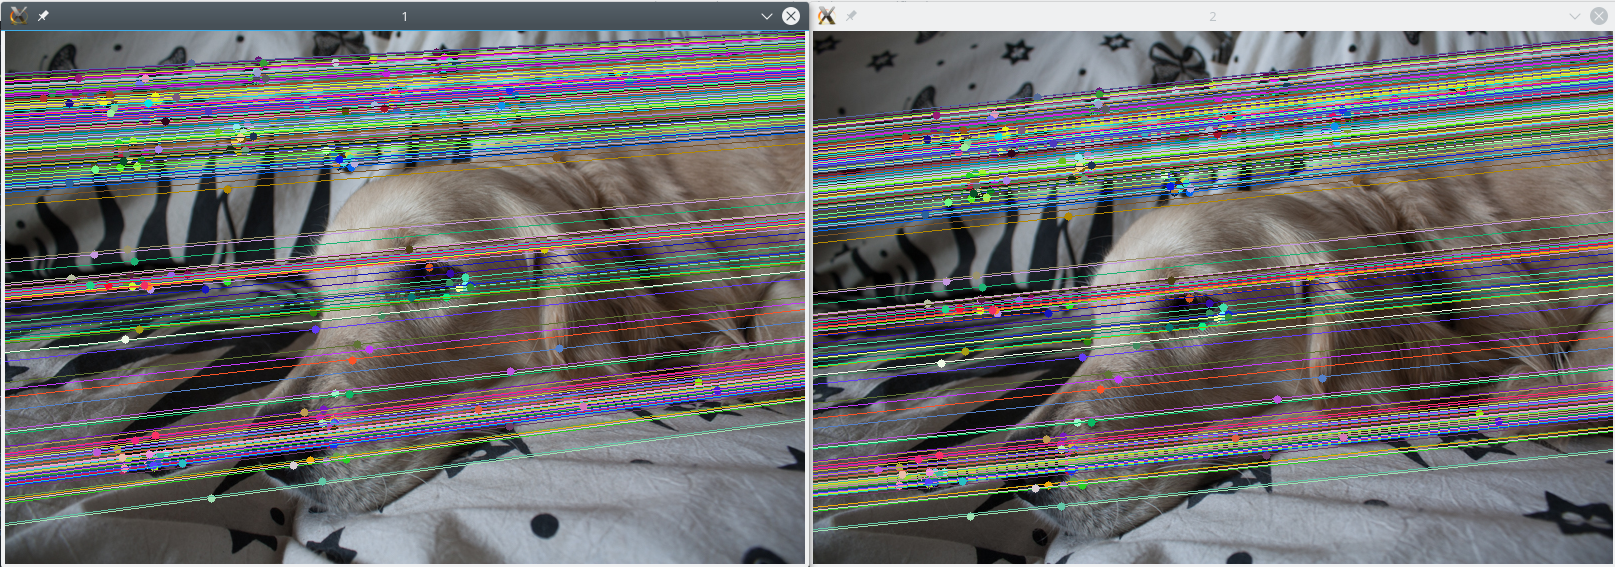
\includegraphics[width=0.8\textwidth]{../Informe/Lola-Normal.png}
              \end{figure}

              \begin{columns}
                \begin{column}{0.2\textwidth}
                  \begin{align*}
                    z &= 0.478684 \\
                    f'(z) &= 267.276
                  \end{align*}
                \end{column}
                \begin{column}{0.8\textwidth}
                  Epipolo

                  $[5868.93; -278.987; 1]$
                \end{column}
              \end{columns}


              }
              \only<2->{\begin{figure}[ht!]
                  \centering
                  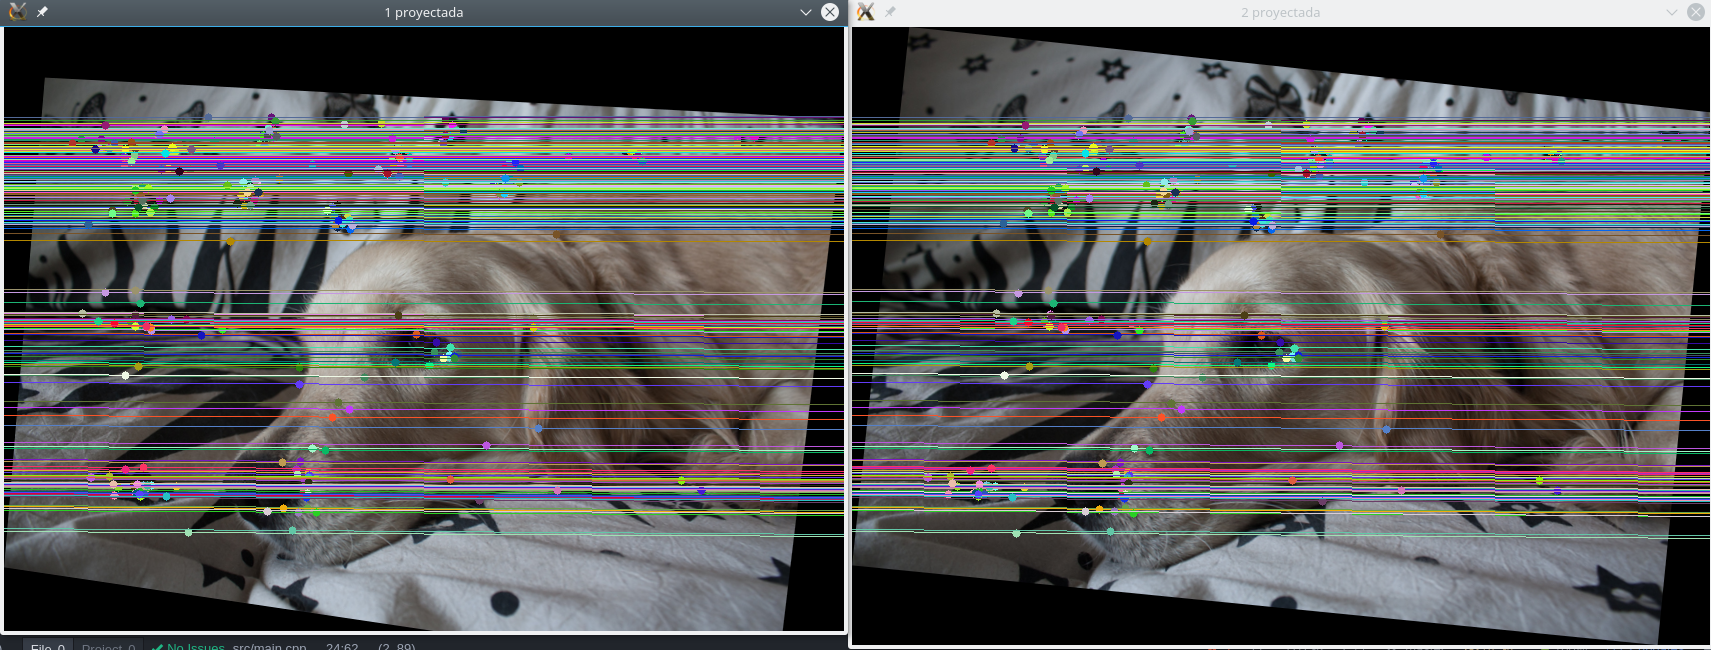
\includegraphics[width=0.8\textwidth]{../Informe/Lola-Proyectado.png}

              \end{figure}
              \begin{columns}
                \begin{column}{0.2\textwidth}
                  \begin{align*}
                    z &= 0.255829 \\
                    f'(z) &= 0
                  \end{align*}

                \end{column}
                \begin{column}{0.8\textwidth}
                  Epipolo

                  $[0.999998; -0.002162; -1.76364e-05]$
                \end{column}
              \end{columns}

              }

          \end{overlayarea}
      \end{frame}

      \begin{frame}{Pruebas y valoración de resultados}{Prueba 2}
        \begin{overlayarea}{\textwidth}{8cm}
            \only<1> {\begin{figure}[ht!]
              \centering
              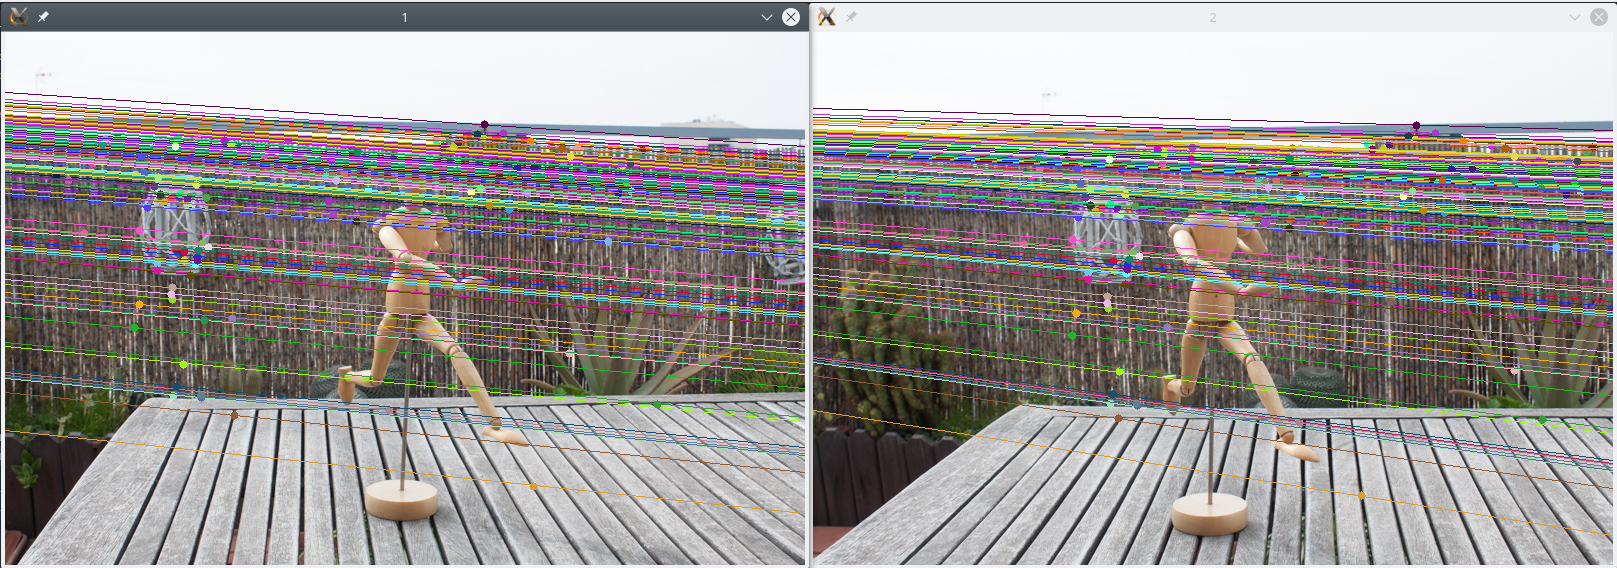
\includegraphics[width=0.8\textwidth]{../Informe/Monigote-Normal.png}
            \end{figure}

            \begin{columns}
              \begin{column}{0.2\textwidth}
                \begin{align*}
                  z &= -0.0225596 \\
                  f'(z) &= 110.449
                \end{align*}
              \end{column}
              \begin{column}{0.8\textwidth}
                Epipolo

                $[-9167.01; -551.777; 1]$
              \end{column}
            \end{columns}


            }
            \only<2->{\begin{figure}[ht!]
                \centering
                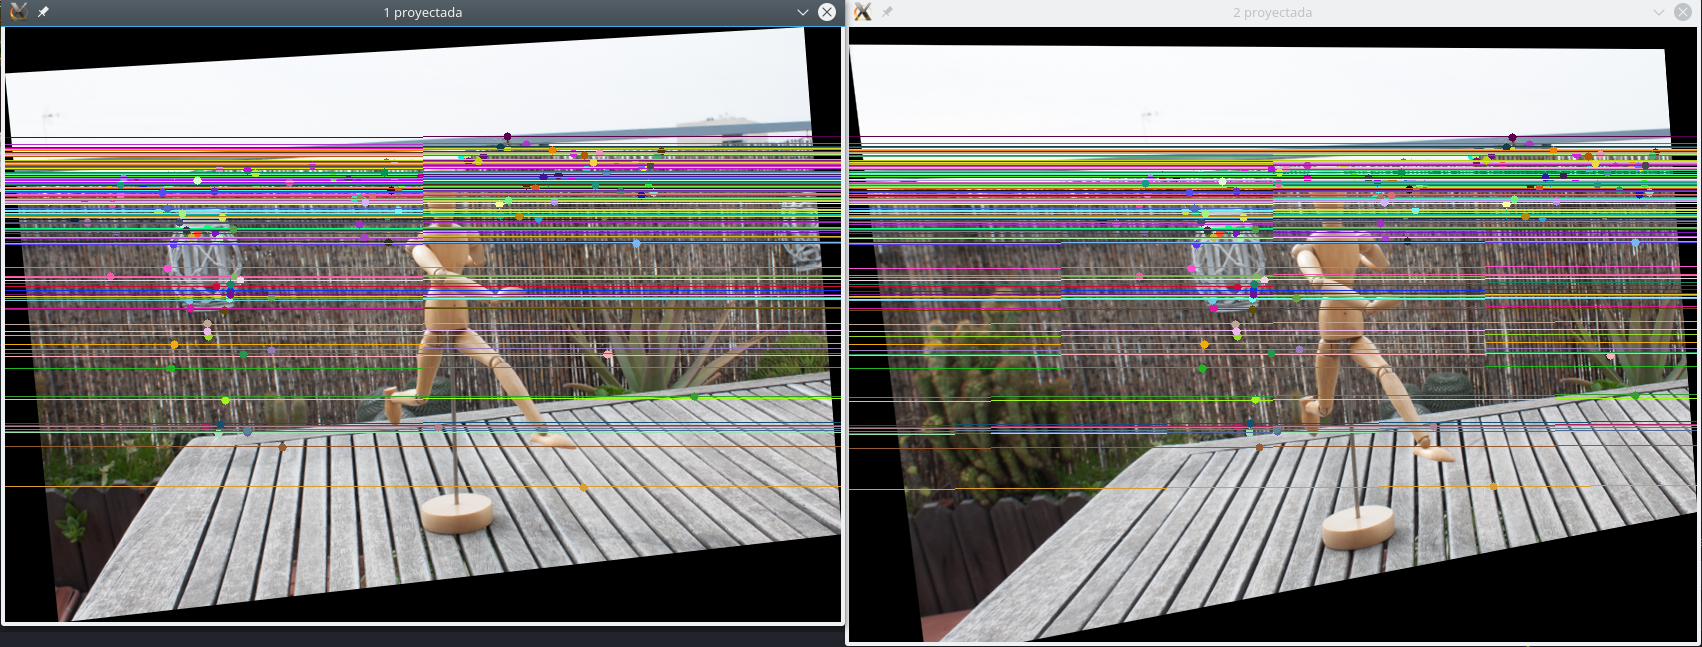
\includegraphics[width=0.8\textwidth]{../Informe/Monigote-Proyectado.png}

            \end{figure}
            \begin{columns}
              \begin{column}{0.2\textwidth}
                \begin{align*}
                  z &= -0.275237 \\
                  f'(z) &= 7.10543e-15
                \end{align*}

              \end{column}
              \begin{column}{0.8\textwidth}
                Epipolo

                $[0.9999; -0.0014679; -2.12774e-06]$
              \end{column}
            \end{columns}

            }

        \end{overlayarea}

      \end{frame}

      \begin{frame}{Pruebas y valoración de resultados}{Prueba 3}

        \begin{overlayarea}{\textwidth}{8cm}
            \only<1> {\begin{figure}[ht!]
              \centering
              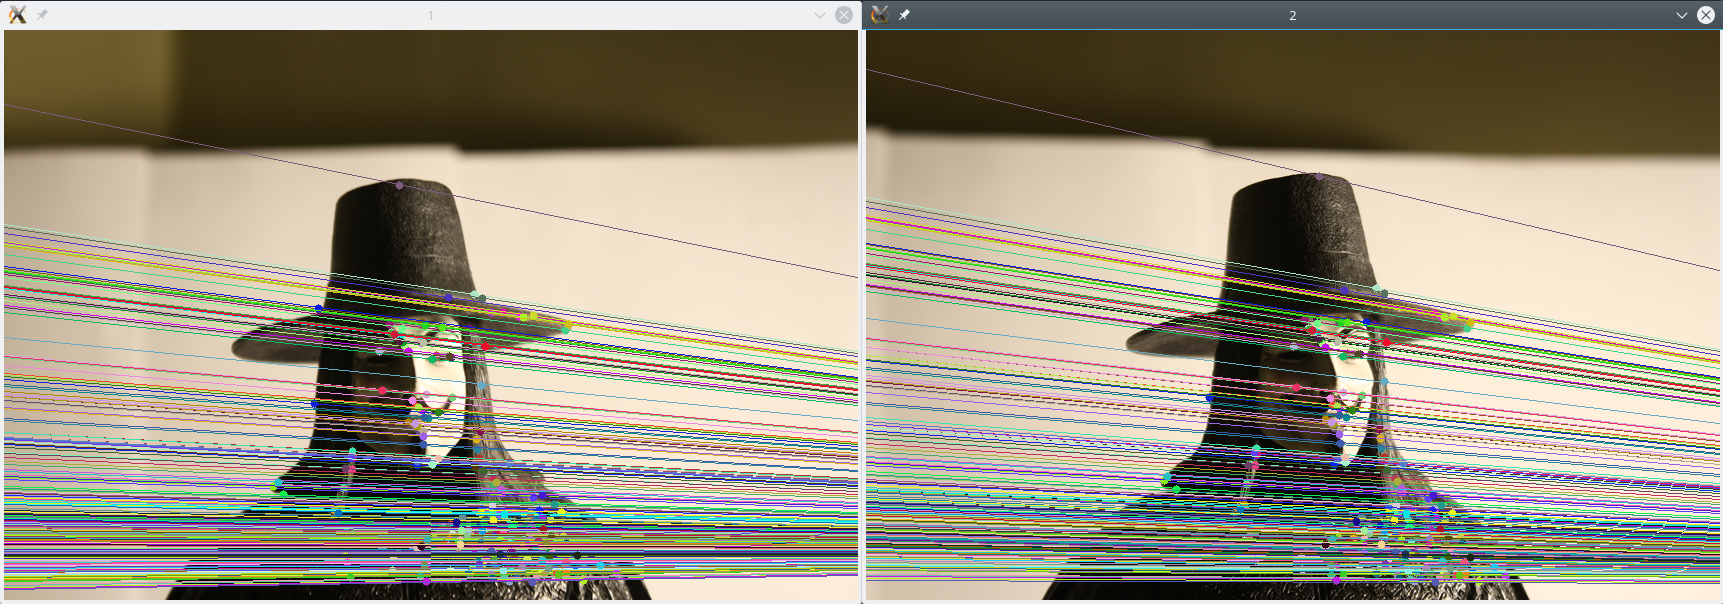
\includegraphics[width=0.7\textwidth]{../Informe/V-Normal.png}
            \end{figure}

            \begin{columns}
              \begin{column}{0.2\textwidth}
                \begin{align*}
                  z &= 0.34294 \\
                  f'(z) &= 10958.3
                \end{align*}
              \end{column}
              \begin{column}{0.8\textwidth}
                Epipolo

                $[2214.98; 523.468; 1]$
              \end{column}
            \end{columns}


            }
            \only<2->{\begin{figure}[ht!]
                \centering
                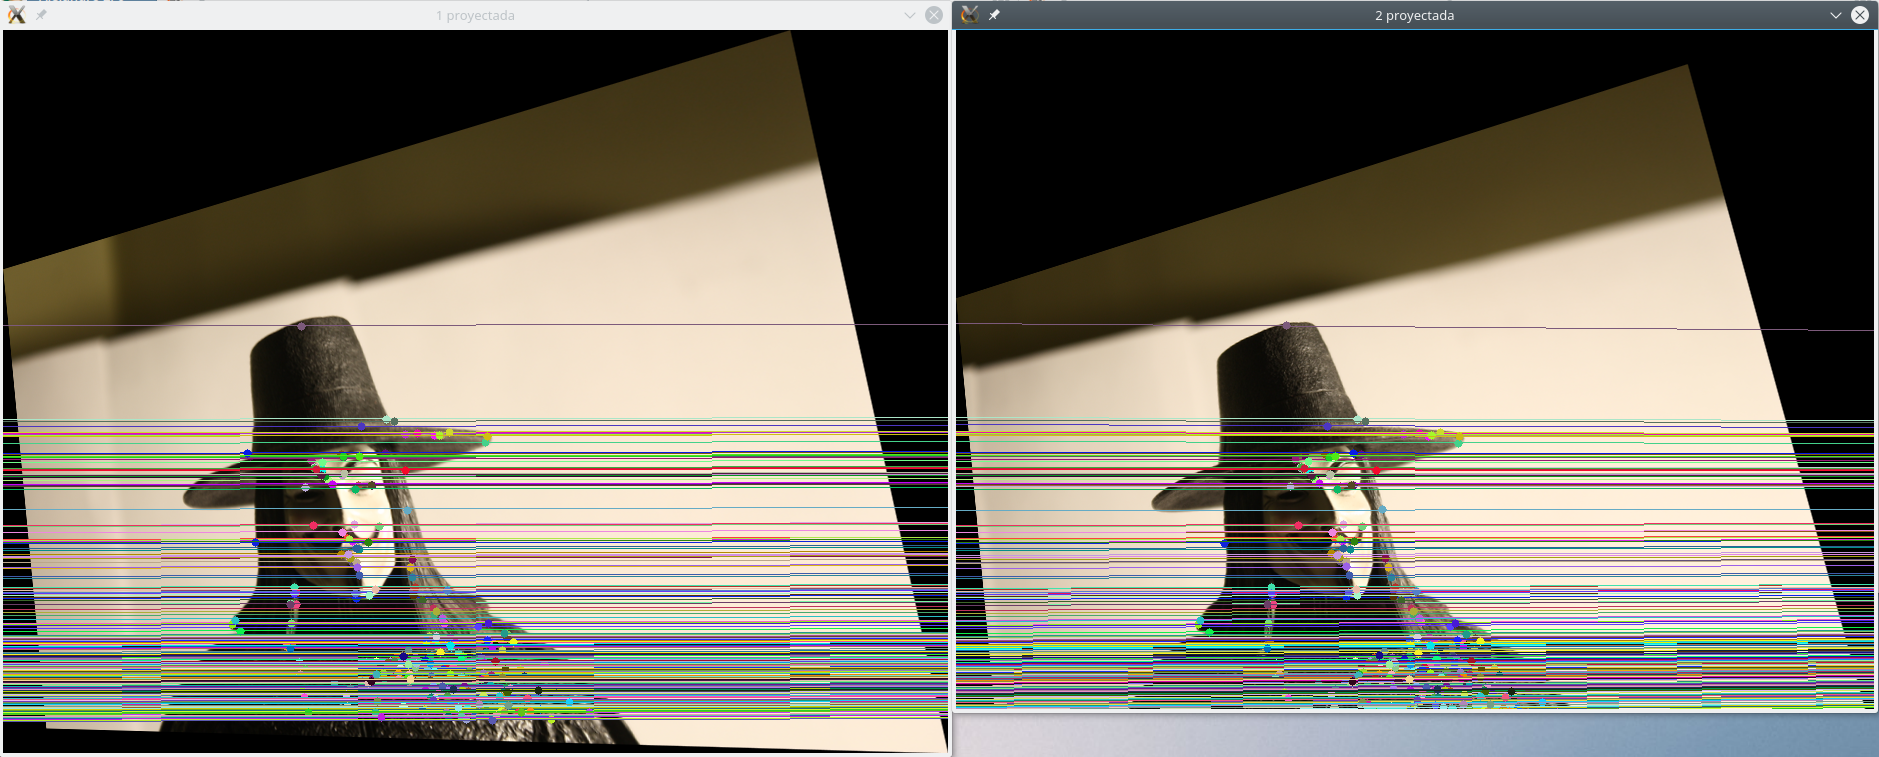
\includegraphics[width=0.7\textwidth]{../Informe/V-Proyectado.png}

            \end{figure}
            \begin{columns}
              \begin{column}{0.2\textwidth}
                \begin{align*}
                  z &= -0.262589 \\
                  f'(z) &= 0
                \end{align*}

              \end{column}
              \begin{column}{0.8\textwidth}
                Epipolo

                $[0.999999; 0.00120902; 7.31557e-06]$
              \end{column}
            \end{columns}

            }

        \end{overlayarea}
      \end{frame}

    \section{Conclusiones}

    \begin{frame}{Conclusiones}

      \begin{itemize}
        \item Problemas de precisión: la descomposición de Cholesky podía fallar debido a que parecía haber valores propios muy pequeños negativos.
        \item Aunque en el artículo se dice que la primera aproximación de $z$ es cercana a la óptima, el método de \emph{Newton-Raphson} nos dice lo contrario: en algunos casos hay un orden de magnitud de diferencia.
        \item Las comprobaciones matemáticas de las ecuaciones que definen la minimización de la distorsión prueban la correcta implementación del algoritmo.
      \end{itemize}
    \end{frame}

    \begin{frame}[plain]
      \huge{GRACIAS}
      \vspace{2mm}
      \hrule
    \end{frame}

\end{document}
